\section{ハミルトニアンの基底変換}
ここでは、Hamiltonianのs変換を行う。
\begin{equation}
    \hat{\mathcal{H}}=\hbar\left(\hat{a}^{\dagger }\ \hat{b}^{\dagger }\right)\left(\begin{array}{cc}
    \tilde{\omega}_{a} & g(\Phi ) \\
    g(\Phi ) & \hat{\omega}_{b}
    \end{array}\right)\left(\begin{array}{l}
    \hat{a} \\
    \hat{b}
    \end{array}\right)
\end{equation}
\begin{equation}
    = \hbar \hat{\omega}_{a} \hat{a}^{\dagger} \hat{a}+\hbar \hat{\omega}_{b} \hat{b}^{\dagger} \hat{b}+\hbar g(\Phi)\left(\hat{a}^{\dagger}\hat{b}+\hat{a} \vec{b}^{+}\right)
\end{equation}
\begin{equation}
    \hat{c}_{\pm}=\frac{\hat{a} \pm \hat{b}}{\sqrt{2}} \quad \hat{c}_{+}^{\dagger}=\frac{\hat{a}^{\dagger} \pm \hat{b}^{\dagger}}{\sqrt{2}}
\end{equation}
\begin{equation}
    \hat{a}^{\dagger}=\frac{\hat{c}_{+}^{\dagger}+\hat{c}_{-}^{\dagger}}{\sqrt{2}} \quad \hat{b}=\frac{\hat{c}_{+}^{\dagger}-\hat{c}_{-}^{\dagger}}{\sqrt{2}}
\end{equation}
\begin{equation}
    \hat{a}=\frac{\hat{c}_{+}+\hat{c}}{\sqrt{2}} \quad \hat{b}=\frac{\hat{c}_{+}-\hat{c}_{-}}{\sqrt{2}}
\end{equation}
\begin{equation}
    \hat{a}^{\dagger} \hat{a}=\frac{1}{2}\left(\hat{c}_{+}^{\dagger}+\hat{c}_{-}^{+}\right)\left(\hat{c}_{t}+\hat{c}_{-}\right) \quad \hat{a}^{\dagger} \hat{b}=\frac{1}{2}\left(\hat{c}_{t}^{+}+\hat{c}_{-}^{+}\right)\left(\hat{c}_{+}-\hat{c}_{-}\right)
\end{equation}
\begin{equation}
    \hat{b} \hat{b}=\frac{1}{2}\left(\hat{c}_{t}+\hat{c}_{-}^{+}\right)\left(\hat{c}_{+}-\hat{c}_{-}\right) \quad \hat{a} \hat{b}^{\dagger}-\frac{1}{2}\left(\hat{c}_{t}+\hat{c}_{-}\right)\left(\hat{c}_{t}^{+}-\hat{c}_{-}^{+}\right)
\end{equation}
\begin{equation}
    \hat{a}^{\dagger} \hat{a}=\frac{1}{2}\left[\hat{c}_{t}^{+} \hat{c}_{+}+\hat{c}_{t}^{+} \hat{c}+\hat{c}_{-}^{+} \hat{c}_{t}+\hat{c}_{-}^{+} \hat{c}_{-}\right]
\end{equation}
\begin{equation}
    \hat{b}^{\dagger} \hat{b}=\frac{1}{2}\left[\hat{c}_{t}^{*} \hat{c}_{t}-\hat{c}_{t}^{n} \hat{c}-\hat{c}_{-}^{+} \hat{c}_{t}+\hat{c}_{-}^{+} \hat{c}-\right]
\end{equation}
\begin{equation}
    \hat{a}^{\dagger} \hat{b}=\frac{1}{2}\left[\dot{c}+\hat{c}_{t}-\hat{c}_{t} \hat{c}_{-}+\hat{c}_{-}^{+} \hat{c}_{t}-\hat{c}_{-}^{\prime} \hat{c}_{-}\right]
\end{equation}
\begin{equation}
    \hat{a} \hat{b}^{\dagger}=\frac{1}{2}\left[\hat{c}_{+} \hat{c}_{+}^{4}-\hat{c}_{+} \hat{c} \pm+\hat{c}-\hat{c}_{+}^{2}-\hat{c}-\hat{c}_{-}\right]
\end{equation}
\begin{equation}
    \hat{H}=\frac{\hbar}{2} \hat{w}_{a}\left[\hat{c}_{t}^{+} \hat{c}_{+}+\hat{c}_{t}^{+} \hat{c}+\hat{c}_{-}^{+} \hat{c}_{t}+\hat{c}_{-}^{+} \hat{c}_{-}\right]
\end{equation}
\begin{equation}
    +\frac{\hbar}{2} \hat{\omega}_{b}\left[\hat{c}_{+}^{+} \hat{c}_{+}-\hat{c}_{+}^{+} \hat{c}_{-}-\hat{c}_{-}^{+} \hat{c}_{+}+\hat{c}_{-}^{+} \hat{c}_{-}\right]
\end{equation}
\begin{equation}
    +\frac{\hbar}{2} g\left[2 \hat{c}+\hat{c}_{+}-2 \hat{c}_{-} \hat{c}\right]
\end{equation}
\begin{equation}
    \hat{H}=\frac{\hbar}{2}\left(\hat{\omega}_{a}+\hat{\omega}_{b}+2 g(\Phi)\right) \hat{c}_{t}^{+} \hat{c}_{+}+\frac{\hbar}{2}\left(\hat{w} a+\hat{w}_{b}-2 g(\Phi)\right) \hat{c}_{-}^{+} \hat{c}_{-}
\end{equation}
\begin{equation}
    +\frac{\hbar}{2} A\left(\hat{w}_{a}-\hat{w}_{b}\right)\left(\hat{c}_{t}+\hat{c}_{-}+\hat{c}_{+} \hat{c}_{-}\right)
\end{equation}
\begin{equation}
    \omega_{a}+\bar{c}_{b}+2 g(\Phi)=\Omega+
\end{equation}
\begin{equation}
    \omega_{a}+\bar{c}_{b}-2 g(\Phi)=\Omega-
\end{equation}
\begin{equation}
    \hat{\omega}_{a}-\hat{w}_{b}=\Delta
\end{equation}
\begin{equation}
    \hat{H}=\frac{\hbar}{2} \Omega+\hat{c}+\hat{c}+\frac{\hbar}{2} \Omega-\hat{c} \pm \hat{c}+\frac{\hbar}{2} \Delta\left(\hat{c}+\hat{c}+\hat{c}_{+} \hat{c}_{-}^{+}\right)
\end{equation}
\begin{equation}
    -\frac{\hbar}{2}\left(\begin{array}{cc}
    \hat{c}_{+} & \hat{c} \pm
    \end{array}\right)\left(\begin{array}{cc}
    \Omega_{1} & \Delta \\
    2 & \Omega_{2}
    \end{array}\right)\left(\begin{array}{l}
    \hat{c}_{+} \\
    \hat{c}_{-}
    \end{array}\right)
\end{equation}
\section{ミアンダインダクタンス}
\section{rf-SQUIDの相互インダクタンス}
dc-SQUIDのインダクタンスは
\begin{equation}
    L_{s}(\Phi)=\frac{\Phi_0}{4\pi I_{c}|{\cos({\phi_{-}^{min}(\Phi_{ext})}})|}
\end{equation}
と記述することができる。
\begin{equation}
    \Phi=\Phi_{ext}+L_{loop}
\end{equation}
\begin{equation}
    \beta_{dc}=\frac{2\pi L_{loop} I_{c}}{\Phi_{0}}
\end{equation}
とすると。
\section{インターデジタルキャパシタンス}
インターデジタルキャパシタンスとは図中の共振器の櫛状になっている部分の構造である。
\begin{figure}[H]
    \centering
    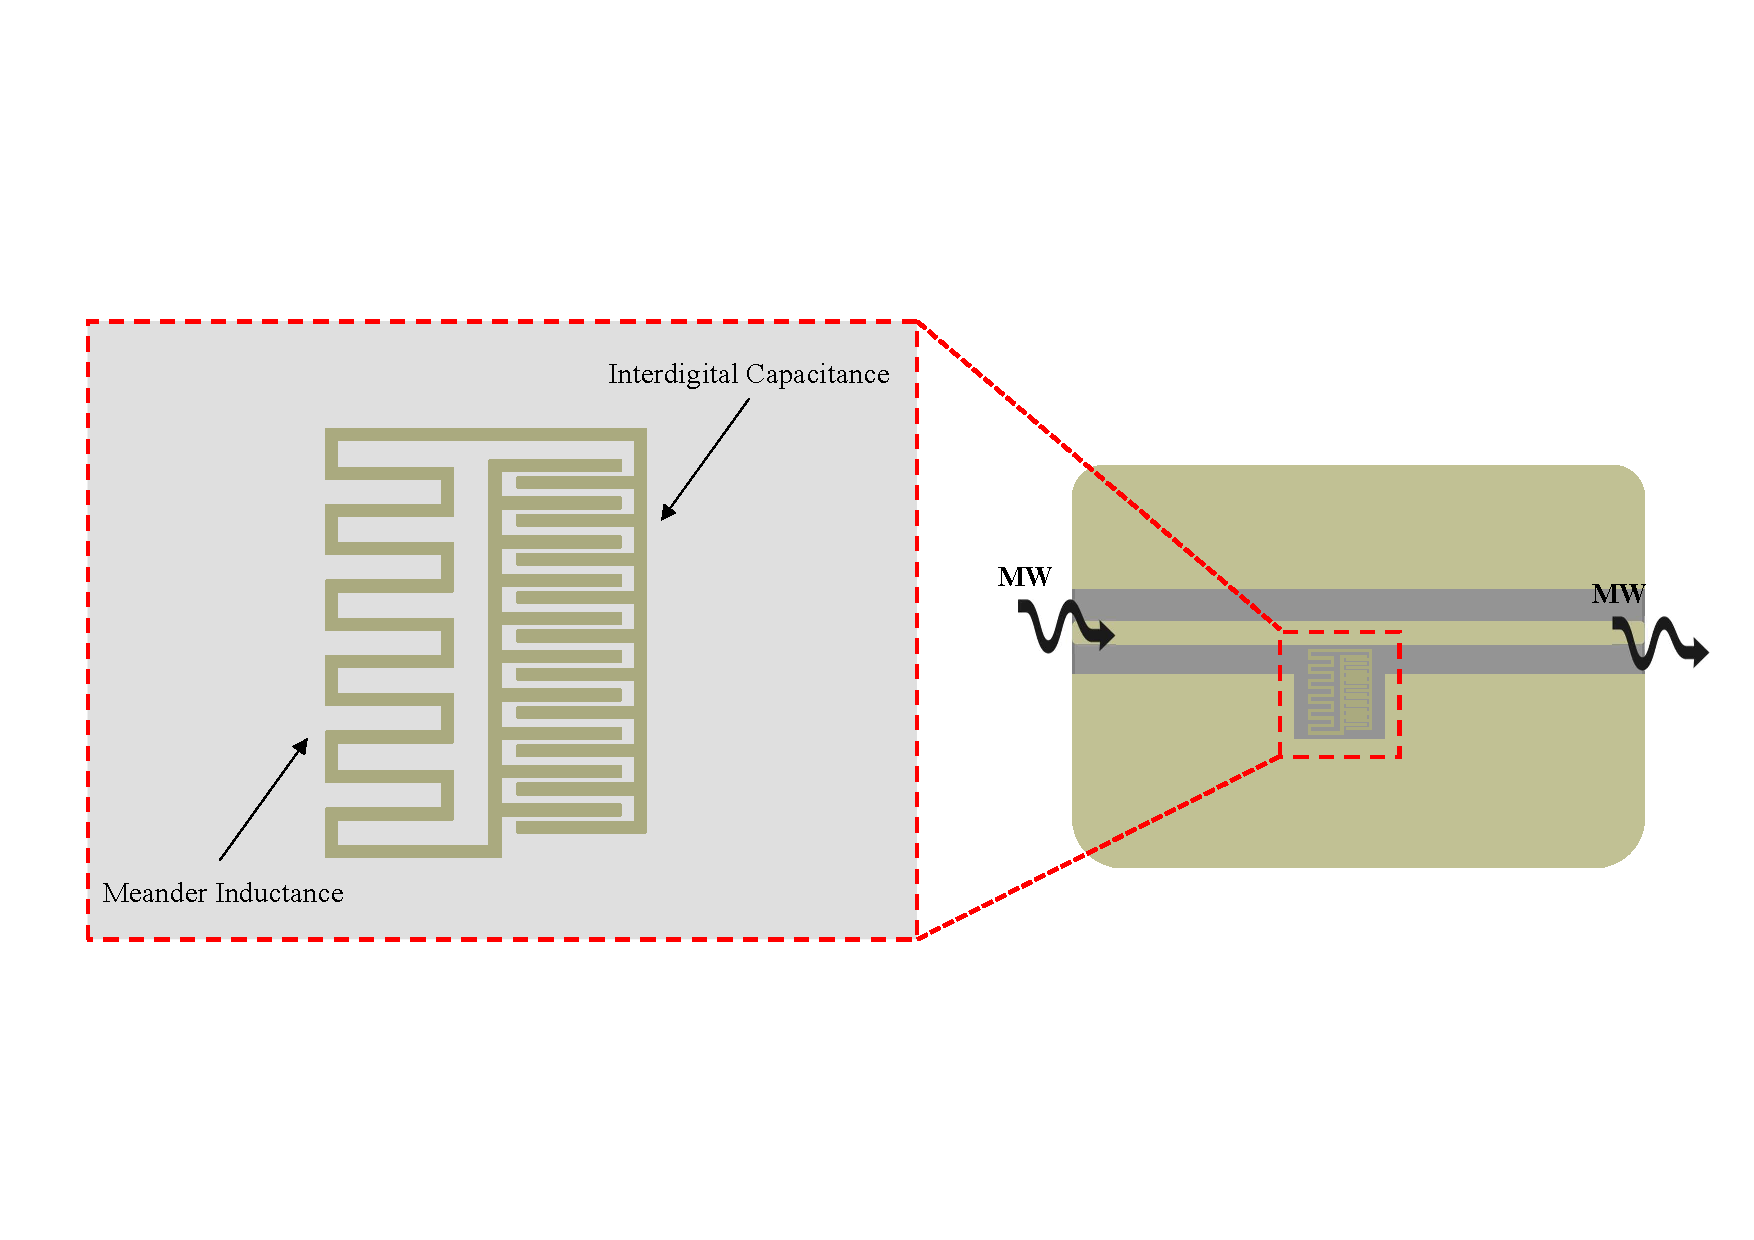
\includegraphics[width=16cm]{lumpedelement.pdf}
    \caption{準集中定数型共振器(再掲)}
\end{figure}
この構造により、電極同士の表面積を上げることでキャパシタンスを増幅することができる。ここではインターデジタルキャパシタンスの計算方法について解説を行う。また、ここで解説するインターデジタルキャパシタンスの計算方法は櫛の数が2本以上のケースである。\cite*{Gevorgian1996,Dib2005,Dib2001ComprehensiveSO}
\begin{figure}[H]
    \centering
    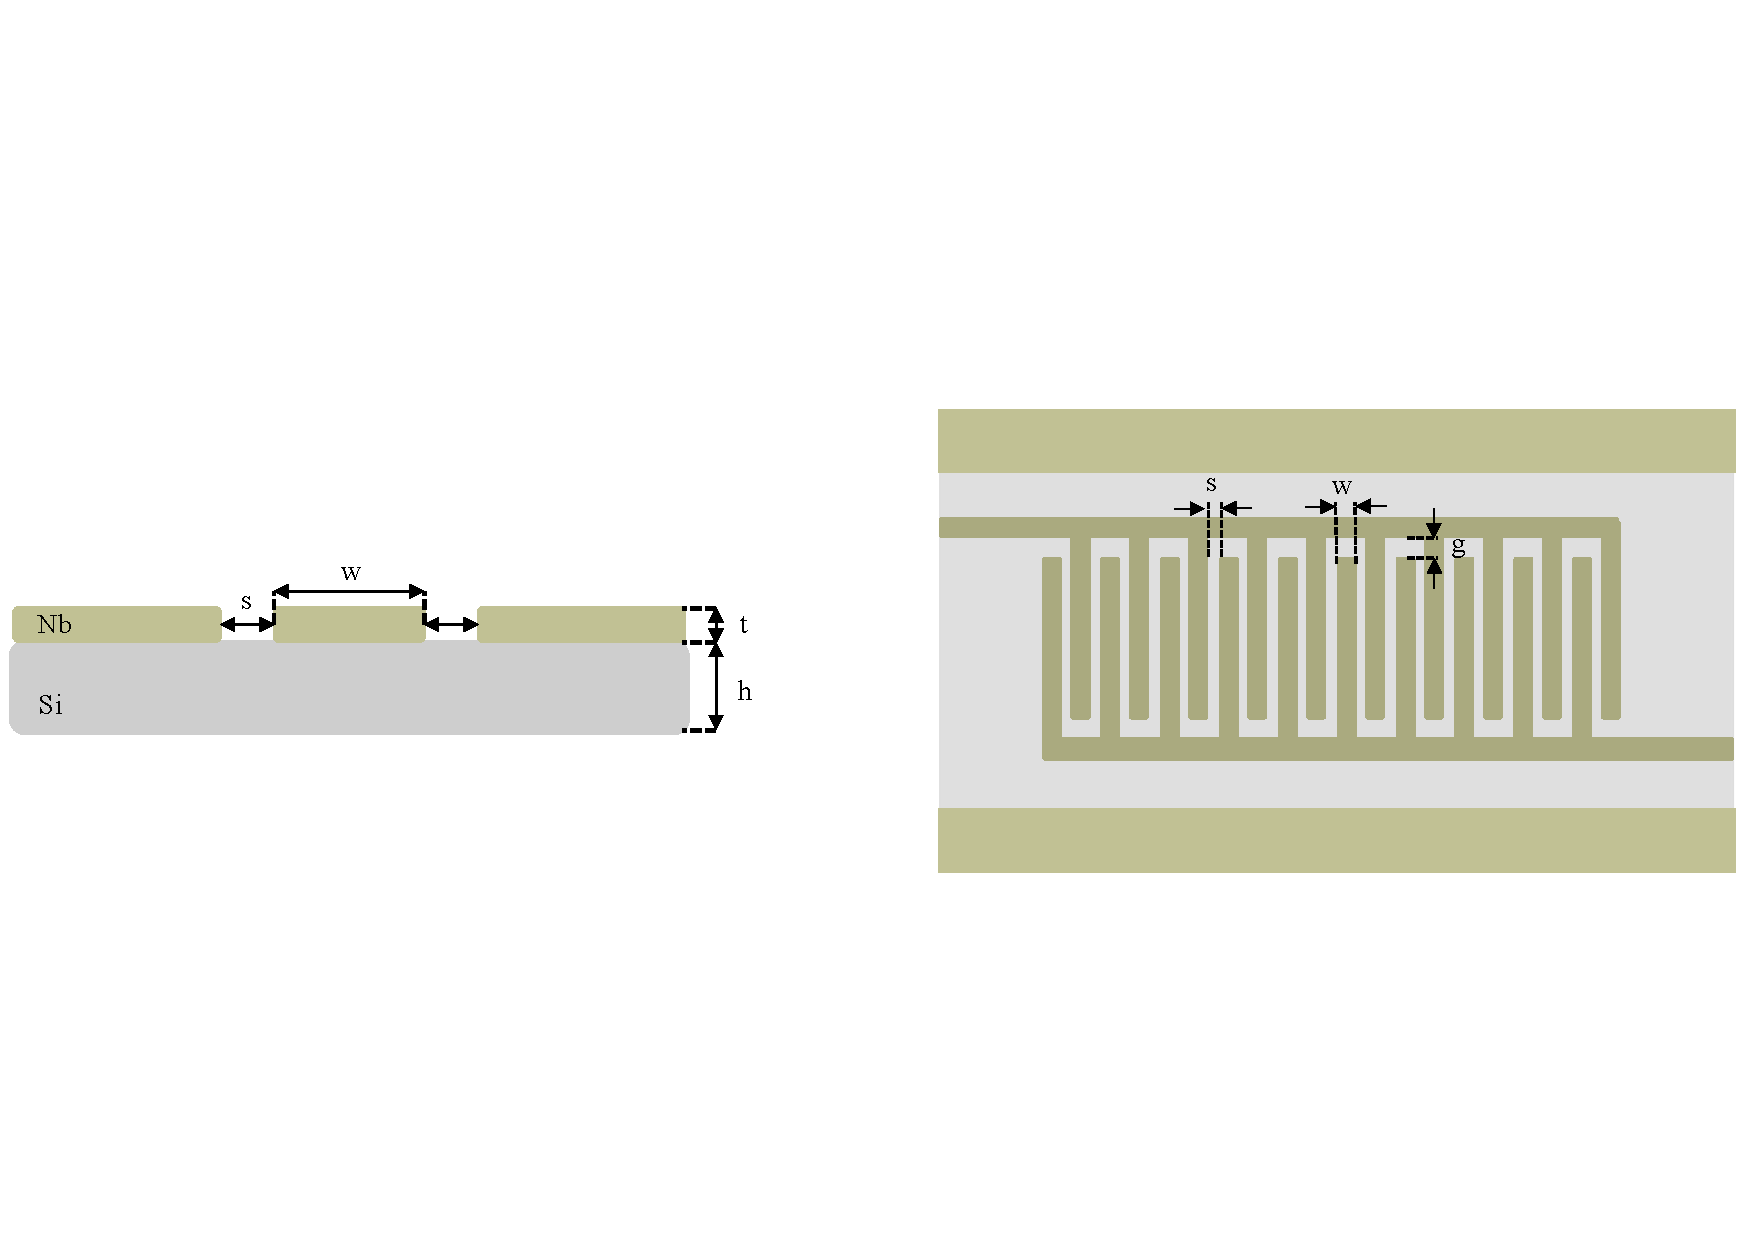
\includegraphics[width=12cm]{IDC2.pdf}
    \caption{インターデジタルキャパシタンス}
\end{figure}
式中の文字は上記の図中のパラメータに対応している。
まず線路の幅wは導体の厚さを含めた実行幅$w_eff$へと変換を行う。\cite*{Gevorgian1996}
\begin{equation}
    W_{e f f}=W+\frac{t}{\pi}\left[1+\ln \left(\frac{4 \pi W}{t}\right)\right]
\end{equation}
ここで相対する導体間のキャパシタンスをCsとする。
キャパシタンスCsを構成するのは櫛が3本であることを想定したキャパシタンスC3、櫛の本数Nに相当するキャパシタンス開放状態になっている最両端の櫛のキャパシタンスCendの3つである。
\begin{equation}
    C_{s}=C_{3}+C_{N}+C_{\text { end }}
\end{equation}
それぞれのキャパシタンスはコンフォーマルマッピングを用いて解析的に求めることが可能である。それぞれの値を求めるにはまずC3について
\begin{equation}
    C_{3}=4 \varepsilon_{0} \varepsilon_{e} \frac{K\left(k_{1}\right)}{K\left(k_{1}^{\prime}\right)} L
\end{equation}\begin{equation}
    \varepsilon_{e}=1+q_{1} \frac{\varepsilon_{r}-1}{2}
\end{equation}
\begin{equation}
        q_{1}=\frac{K\left(k_{1}^{\prime}\right)}{K\left(k_{1}\right)} \frac{K\left(k_{2}\right)}{K\left(k_{2}^{\prime}\right)}
\end{equation}
\begin{equation}
    k_{1}=\frac{W}{W+2 S} \sqrt{\frac{1-\left[\frac{W+2 S}{3 W+2 S}\right]^{2}}{1-\left[\frac{W}{3 W+2 S}\right]^{2}}}
\end{equation}
\begin{equation}
    \begin{aligned}
    k_{2}=& \frac{\sinh \left(\frac{\pi W}{4 h}\right)}{\sinh \left(\frac{\pi(W+2 S)}{4 h}\right)} 
    & \sqrt{\frac{\sinh ^{2}\left(\frac{\pi(3 W+2 S)}{4 h}\right)-\sinh ^{2}\left(\frac{\pi(W+2 S)}{4 h}\right)}{\sinh ^{2}\left(\frac{\pi(3 W+2 S)}{4 h}\right)-\sinh ^{2}\left(\frac{\pi W}{4 h}\right)}}
    \end{aligned}
\end{equation}
同様にしてCNについて求めると
\begin{equation}
    C_{N}=(N-3) \varepsilon_{0} \varepsilon_{N} \frac{K\left(k_{3}\right)}{K\left(k_{3}^{\prime}\right)} L
\end{equation}
\begin{equation}
    \varepsilon_{N}=1+q_{N} \frac{\varepsilon_{r}-1}{2}
\end{equation}
\begin{equation}
    q_{N}=\frac{K\left(k_{3}^{\prime}\right)}{K\left(k_{3}\right)} \frac{K\left(k_{4}\right)}{K\left(k_{4}^{\prime}\right)},
\end{equation}
\begin{equation}
    k_{3}=\frac{W}{W+S},
\end{equation}
\begin{equation}
    \begin{aligned}
    k_{4}=& \frac{\sinh \left(\frac{\pi W}{4 h}\right)}{\sinh \left(\frac{\pi(W+ S)}{4 h}\right)} 
    & \sqrt{\frac{\sinh ^{2}\left(\frac{\pi(W+S)}{4 h}\right)+\sinh ^{2}\left(\frac{\pi(W+ S)}{4 h}\right)}{\cosh ^{2}\left(\frac{\pi(W)}{4 h}\right)-\sinh ^{2}\left(\frac{\pi (W+S)}{4 h}\right)}}
    \end{aligned}
\end{equation}
として求まる。最後にCendについて、この計算を行う上で主に参考にしている論文\cite*{Dib2005}ではCendの計算について\cite*{Dib2001ComprehensiveSO}中の式
\begin{equation}
    C_{o c}=c_{e f f} C_{o e}\left(\epsilon_{r}=1\right)
\end{equation}
\begin{equation}
    \label{Cend}
    C_{\alpha c}\left(c_{r}=1\right)=\frac{c_{0}}{\pi}\left[\frac{1}{g^{2}} f_{s}(g, W+S, 0)+\frac{1}{W^{2}} f_{0}(W, S, 0)\right]
\end{equation}
\begin{equation}
    \label{fs}
    \begin{aligned}
    f_{s}(a, b, c) &=\frac{4}{3} c^{3}+f(a, c)+f(b, c)-4 a b c \tan ^{-1}\left(\frac{a b}{c \tau}\right)-\frac{2}{3}\left(b^{2}-2 c^{2}+a^{2}\right) \tau \\
    &+\left(a^{2}-c^{2}\right) b \ln \left(\frac{\tau+b}{\tau-b}\right)+\left(b^{2}-c^{2}\right) a \ln \left(\frac{\tau+a}{\tau-a}\right)
    \end{aligned}
\end{equation}
\begin{equation}
    \label{f0}
    f_{0}(a, b, c) =\frac{4}{3} c^{3}+f(a, c)+f(a+b, c)-\frac{1}{2} f(b+2 a, c)-\frac{1}{2} f(b, c)
\end{equation}
\begin{equation}
    \label{fx}
    f(x, y) =\frac{2}{3}\left(x^{2}-2 y^{2}\right) \sqrt{x^{2}+y^{2}}+y^{2} x \ln \left(\frac{\sqrt{x^{2}+y^{2}}+x}{\sqrt{x^{2}+y^{2}}-x}\right)
\end{equation}
を使用したと記述されているが式\ref*{fx}の第2項目は不適切であるため、本稿では含めずに計算した。というのも式\ref*{fx}が使用されている式\ref{Cend,fs,f0}に注目すると式\label{fx}中の$y$は常にゼロであり、第2項目は2乗でゼロに収束する。よって2項目は計算に含まれないことになる。よって計算には以下
\begin{equation}
    \label{fx_re}
    f(x, y)_{revised} =\frac{2}{3}\left(x^{2}-2 y^{2}\right) \sqrt{x^{2}+y^{2}}
\end{equation}
をもちいた。
以上の計算式を用いてインターデジタルキャパシタンスの値を見積もることができる。
ここではさらに本稿で使用したパラメータを用いて櫛の本数Nに対してキャパシタンスの値がどれだけ変化するのか、また、実験結果との比較を行う。
\begin{figure}[H]
    \centering
    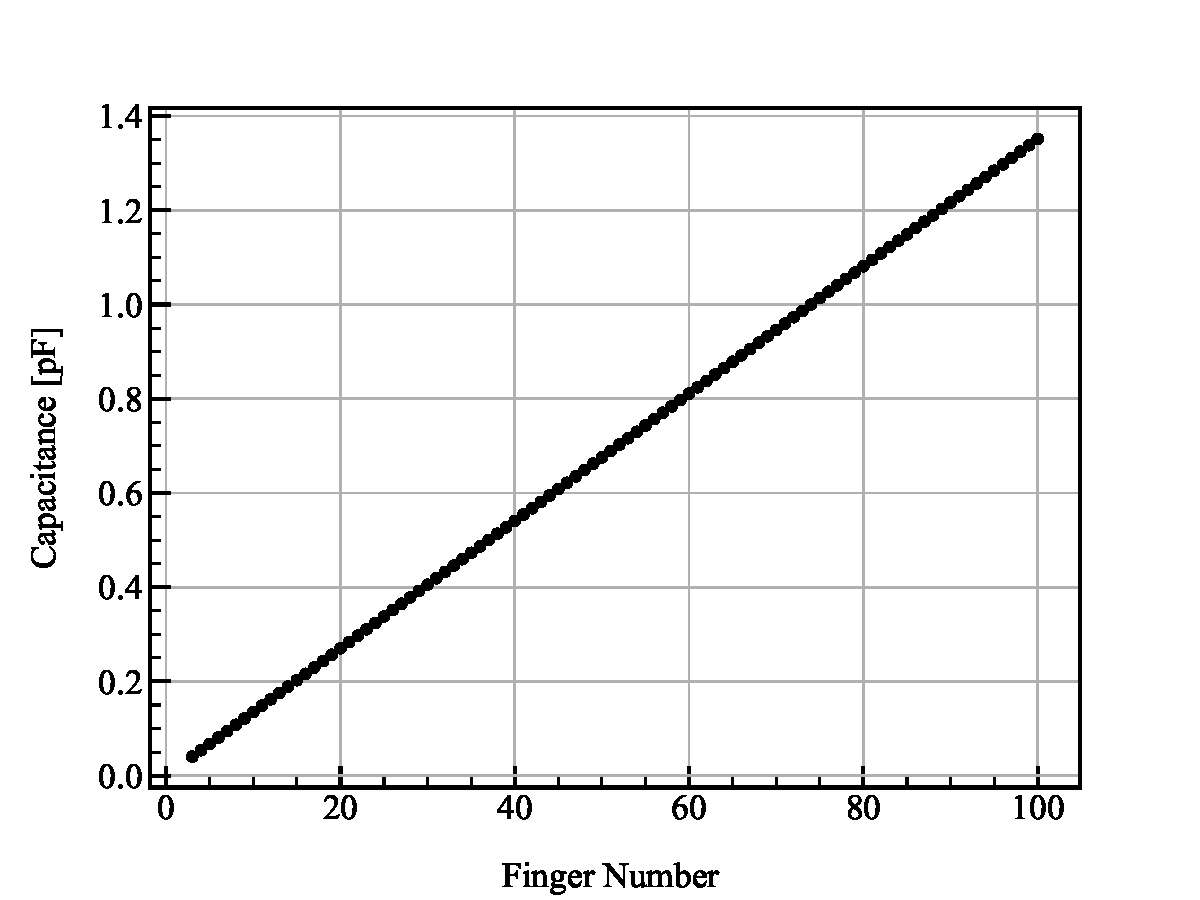
\includegraphics[width=10cm]{IDC_cal.pdf}
    \caption{キャパシタンス vs 櫛の本数}
\end{figure}
\section{マスター方程式}
\section{2点相関関数}
